\chapter{Testing e Benchmarking}

Ai fini di verificare il corretto funzionamento del sistema e valutarne le prestazioni, sono stati sviluppati test e benchmark.
Firegex già presentava un set di tests, che con l'integrazione di nfproxy sono stati ampliati e migliorati, al fine di coprire anche le nuove
feature introdotte.\\
I test sono eseguiti prima di ogni rilascio in automatico, al fine di garantire che le modifiche apportate non abbiano introdotto regressioni.
I rilasci di firegex avvengono tramite GitHub Actions, che ad ogni rilascio su GitHub esegue i test e, in caso di successo,
pubblica il container di firegex sul Github Container Registry (ghcr.io/pwnzer0tt1/firegex) e rilascia una nuova versione della libreria inclusa 
nello stesso repository su PyPi.\\
I rilasci avvengono sia per architetture \texttt{x86\_64} che \texttt{ARM64}, al fine di supportare il maggior numero di dispositivi possibile.\\

\section{Integrazione dei test}

I test sono stati integrati nel repository di firegex, all'interno della cartella \texttt{tests}.\\
I test riguardanti nfproxy sono contenuti nel file \texttt{tests/nfproxy\_test.py}, ed esegue la seguente serie di operazioni:

\begin{itemize}
    \setlength{\itemsep}{5pt}
    \setlength{\parskip}{5pt}
    \item Avvia un nuovo servizio sull'interfaccia di loopback, e verifica che il traffico non sia stato compromesso dal semplice avvio del modulo.
    \item Verifica che ogni tipo di vedict stia correttamente funzionando inserendo un filtro che verifica se sul segmento TCP sia presente un payload specifico.
    Verificando che il traffico si comporti coerentemente al fatto che il payload specifico sia stato scambiato o meno.
    \item Si verifica che il verdict di UNSTABLE\_MANGLE funzioni correttamente, testando sia mangle a pacchetti più piccoli che più grandi, comprovando
    pertanto che la traduzione degli ack e seq avvenga correttamente generando altro traffico a seguito della modifica.
    \item Si asssucura che le funzionalità di interruzione del servizio e del singolo pyfilter sia correttamente funzionante.
    \item Per ogni tipo di datahandler, si scambiano dei payload di prova al fine di verificare se il parsing dei vari dati avvenga correttamente.
    Datahandler testati: \texttt{TCPInputStream}, \texttt{TCPOutputStream}, \texttt{HttpRequest}, \texttt{HttpResponse}, \texttt{HttpRequestHeader},
    \texttt{HttpResponseHeader} includendo anche il parsing di \texttt{Frame websocket}.
    \item Vengono testate tutte le API backend di nfproxy, verificando che le chiamate restituiscano i valori corretti, e si comportino in modo coerente alla loro funzione.
    \item Si verifica inoltre che vengano contate correttamente le connessioni bloccate, e i pacchetti modificati nelle statistiche.
\end{itemize}

\section{Benchmark}

I benchmark sono stati realizzati tramite uno script python con l'ausilio di \texttt{iperf3}\footcite{\url{https://iperf.fr/}}{iperf_website}.\\
Le casistiche utilizzate sono di semplice natura, verificano le prestazioni in termini di throughput, e lo fanno sia a servizio attivo senza filtri, che con
un filtro che applica la seguente regex al payload TCP (regex per il matching di email):
\begin{verbatim}
    (?:[a-z0-9!#$%&'*+/=?^_`{|}~-]+
       (?:\.[a-z0-9!#$%&'*+/=?^_`{|}~-]+)* |
       "(?:[\x01-\x08\x0b\x0c\x0e-\x1f\x21\x23-\x5b\x5d-\x7f] |
           \\[\x01-\x09\x0b\x0c\x0e-\x7f])*")
    @
    (?:(?:[a-z0-9](?:[a-z0-9-]*[a-z0-9])?\.)+
        [a-z0-9](?:[a-z0-9-]*[a-z0-9])? |
       \[(?:(?:25[0-5] | 2[0-4][0-9] | [01]?[0-9][0-9]?)\.){3}
           (?:25[0-5] | 2[0-4][0-9] | [01]?[0-9][0-9]? |
               [a-z0-9-]*[a-z0-9]:
               (?:[\x01-\x08\x0b\x0c\x0e-\x1f\x21-\x5a\x53-\x7f] |
                   \\[\x01-\x09\x0b\x0c\x0e-\x7f])+)\])
\end{verbatim}

Si da per assodato che i filtri siano correttamente funzionanti (la cui caratteristiche è verificata dai test), e si vuole verificare l'overhead causato
dai filtri che comunque vengono eseguiti e che quindi diminuiscono il throughput.\\
I benchmark sono stati eseguiti su una macchina con le seguenti caratteristiche:\\

\texttt{Macbook Air M2 16GB RAM}\\
\texttt{Su una VM avviata da OrbStack con Fedora Linux 41 (Container Image) aarch64}\\
\texttt{Linux 6.12.13-orbstack-00304-gede1cf3337c4}\\

Lo script python creato è creato appositamente per ripetere la stessa misura un numero variabile di volte, sia sul modulo nfproxy, che sul modulo nfregex.
I risultati sono stati raccolti e analizzati, e messi a disposizioni nei grafici seguenti.\\
I benchmark sono stati eseguiti con i seguenti parametri: \texttt{python3 comparemark.py nfproxy -p testpassword -d 1 -s 50 -V 100} e \texttt{python3 comparemark.py nfregex -p testpassword -d 1 -s 50 -V 100}
con 1 secondo di durata del singolo benchmark, 50 connessioni simultanee, e 100 misure eseguite.\\
Il numero indicato dopo la \texttt{T} nei grafici indica il numero di thread con cui firegex è stato configurato: quindi eseguiti sia in
single-threading che in multi-threading (con 8 thread).\\

\begin{figure}[H]
    \centering
    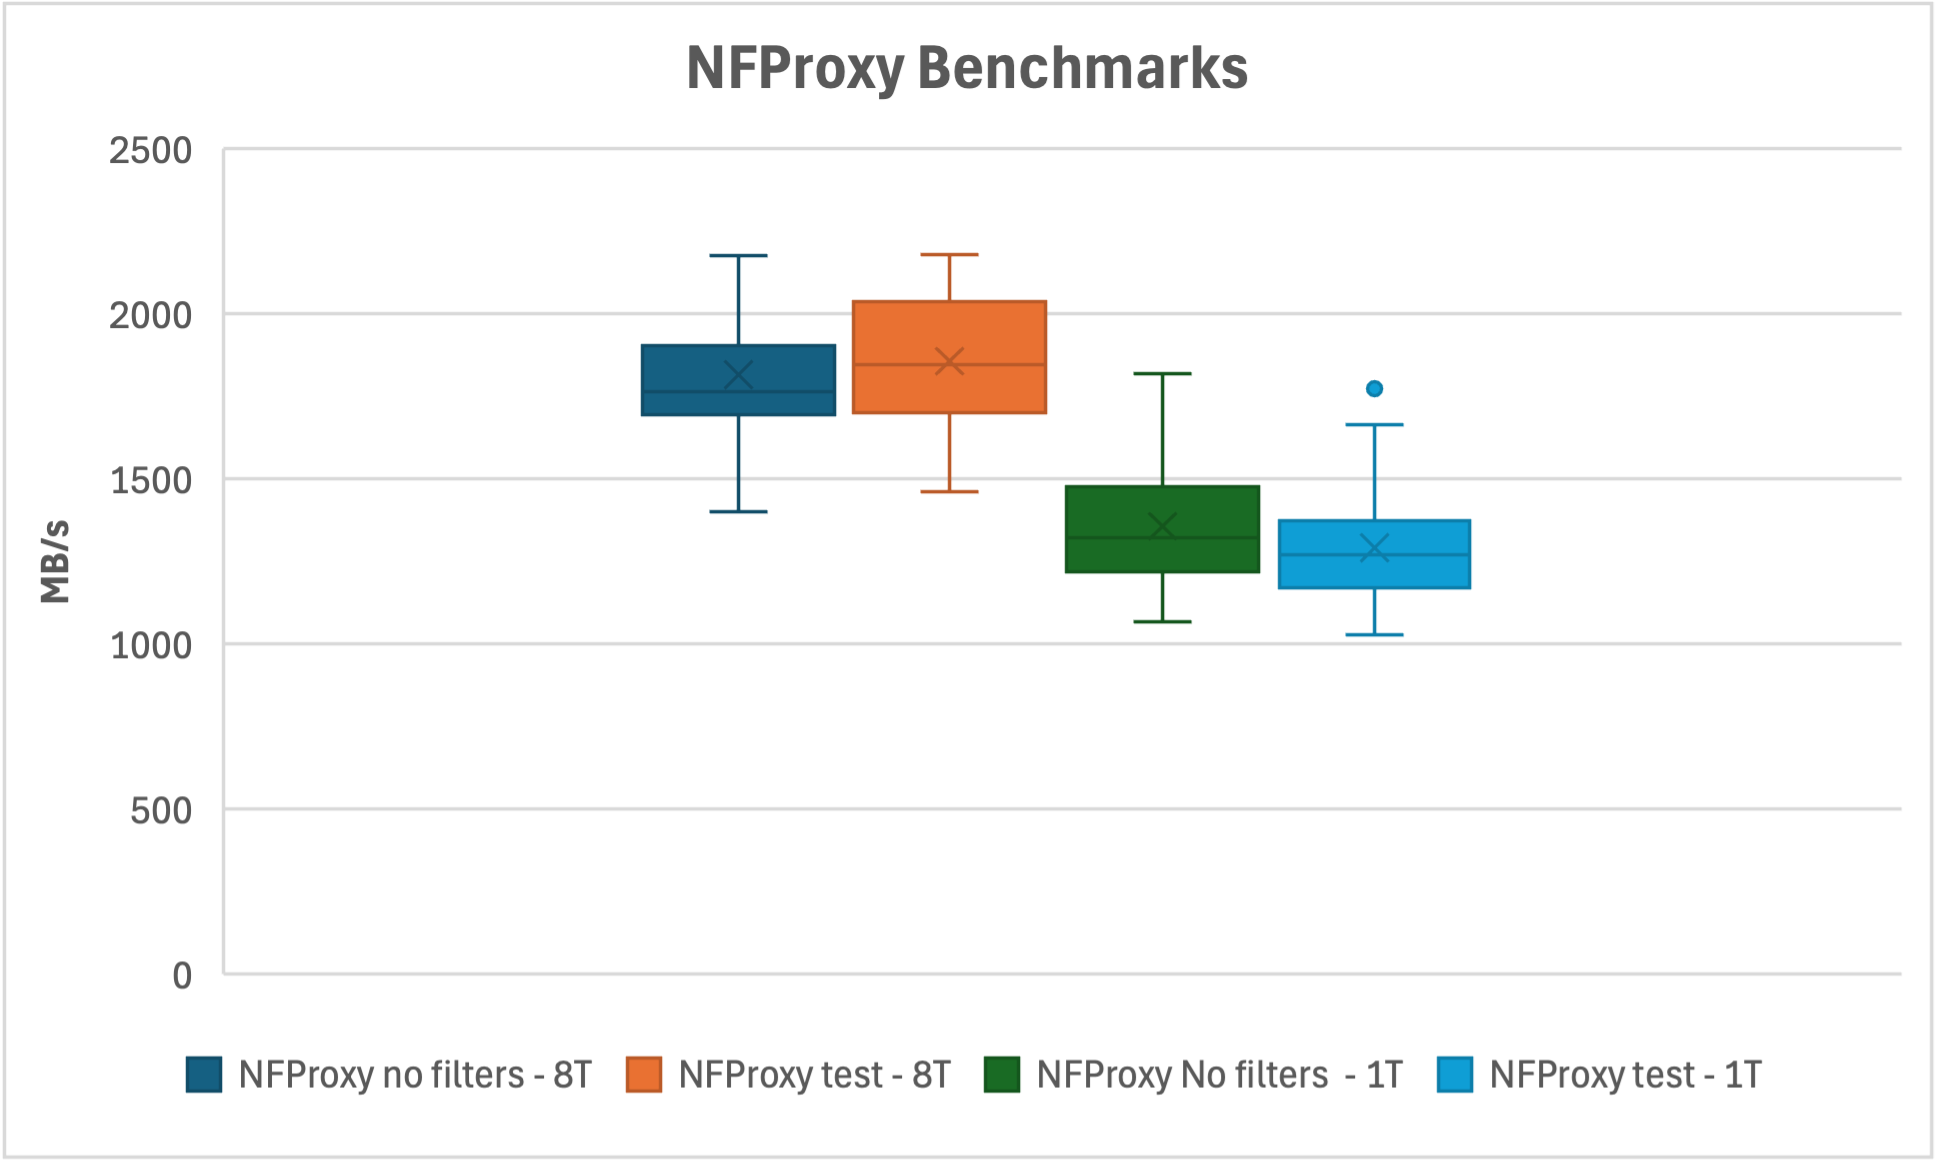
\includegraphics[width=0.98\textwidth]{images/chapter4/whisker_nfproxy.png}
    \caption{Grafico Whisker sulle misure di throughput di nfproxy}\label{fig:wisker_nfproxy}
\end{figure}

\begin{figure}[H]
    \centering
    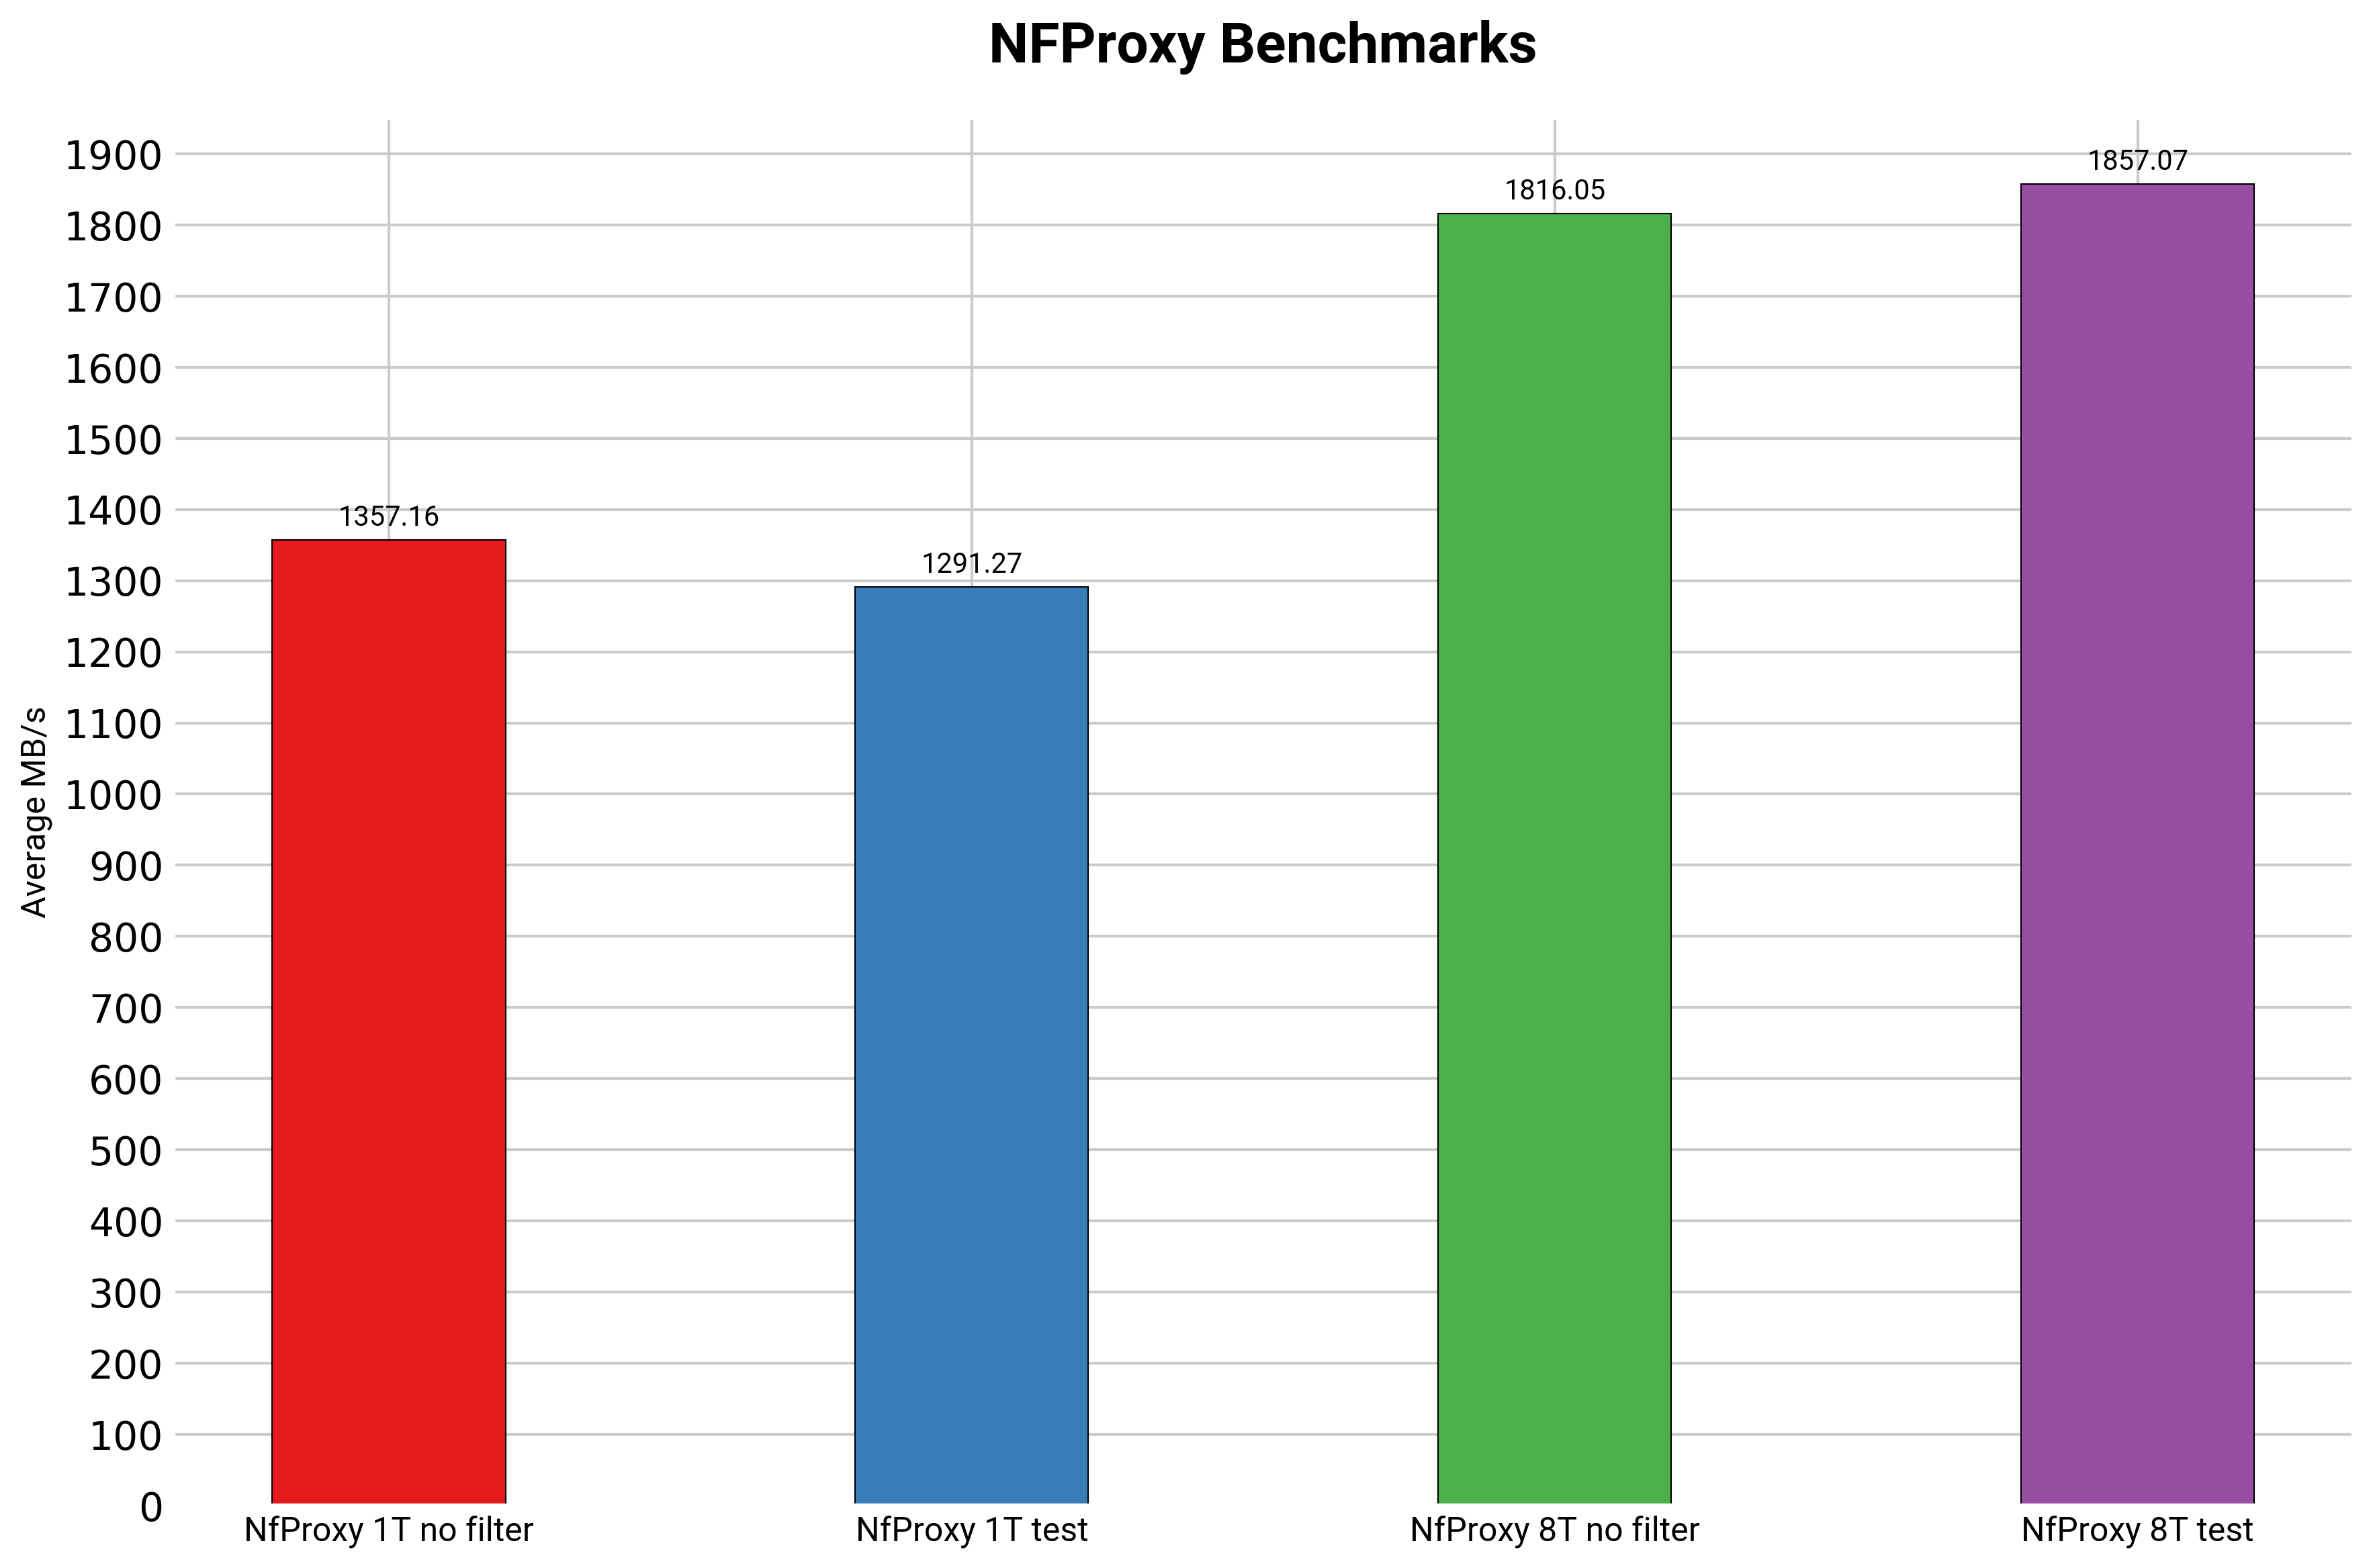
\includegraphics[width=0.98\textwidth]{images/chapter4/istogramma_nfproxy.png}
    \caption{Istogramma sulle misure medie di throughput di nfproxy}\label{fig:istogramma_nfproxy}
\end{figure}

Si può notare come le performance in multi-threading di nfproxy siano migliori rispetto all'utilizzo del singolo thread.

\begin{figure}[H]
    \centering
    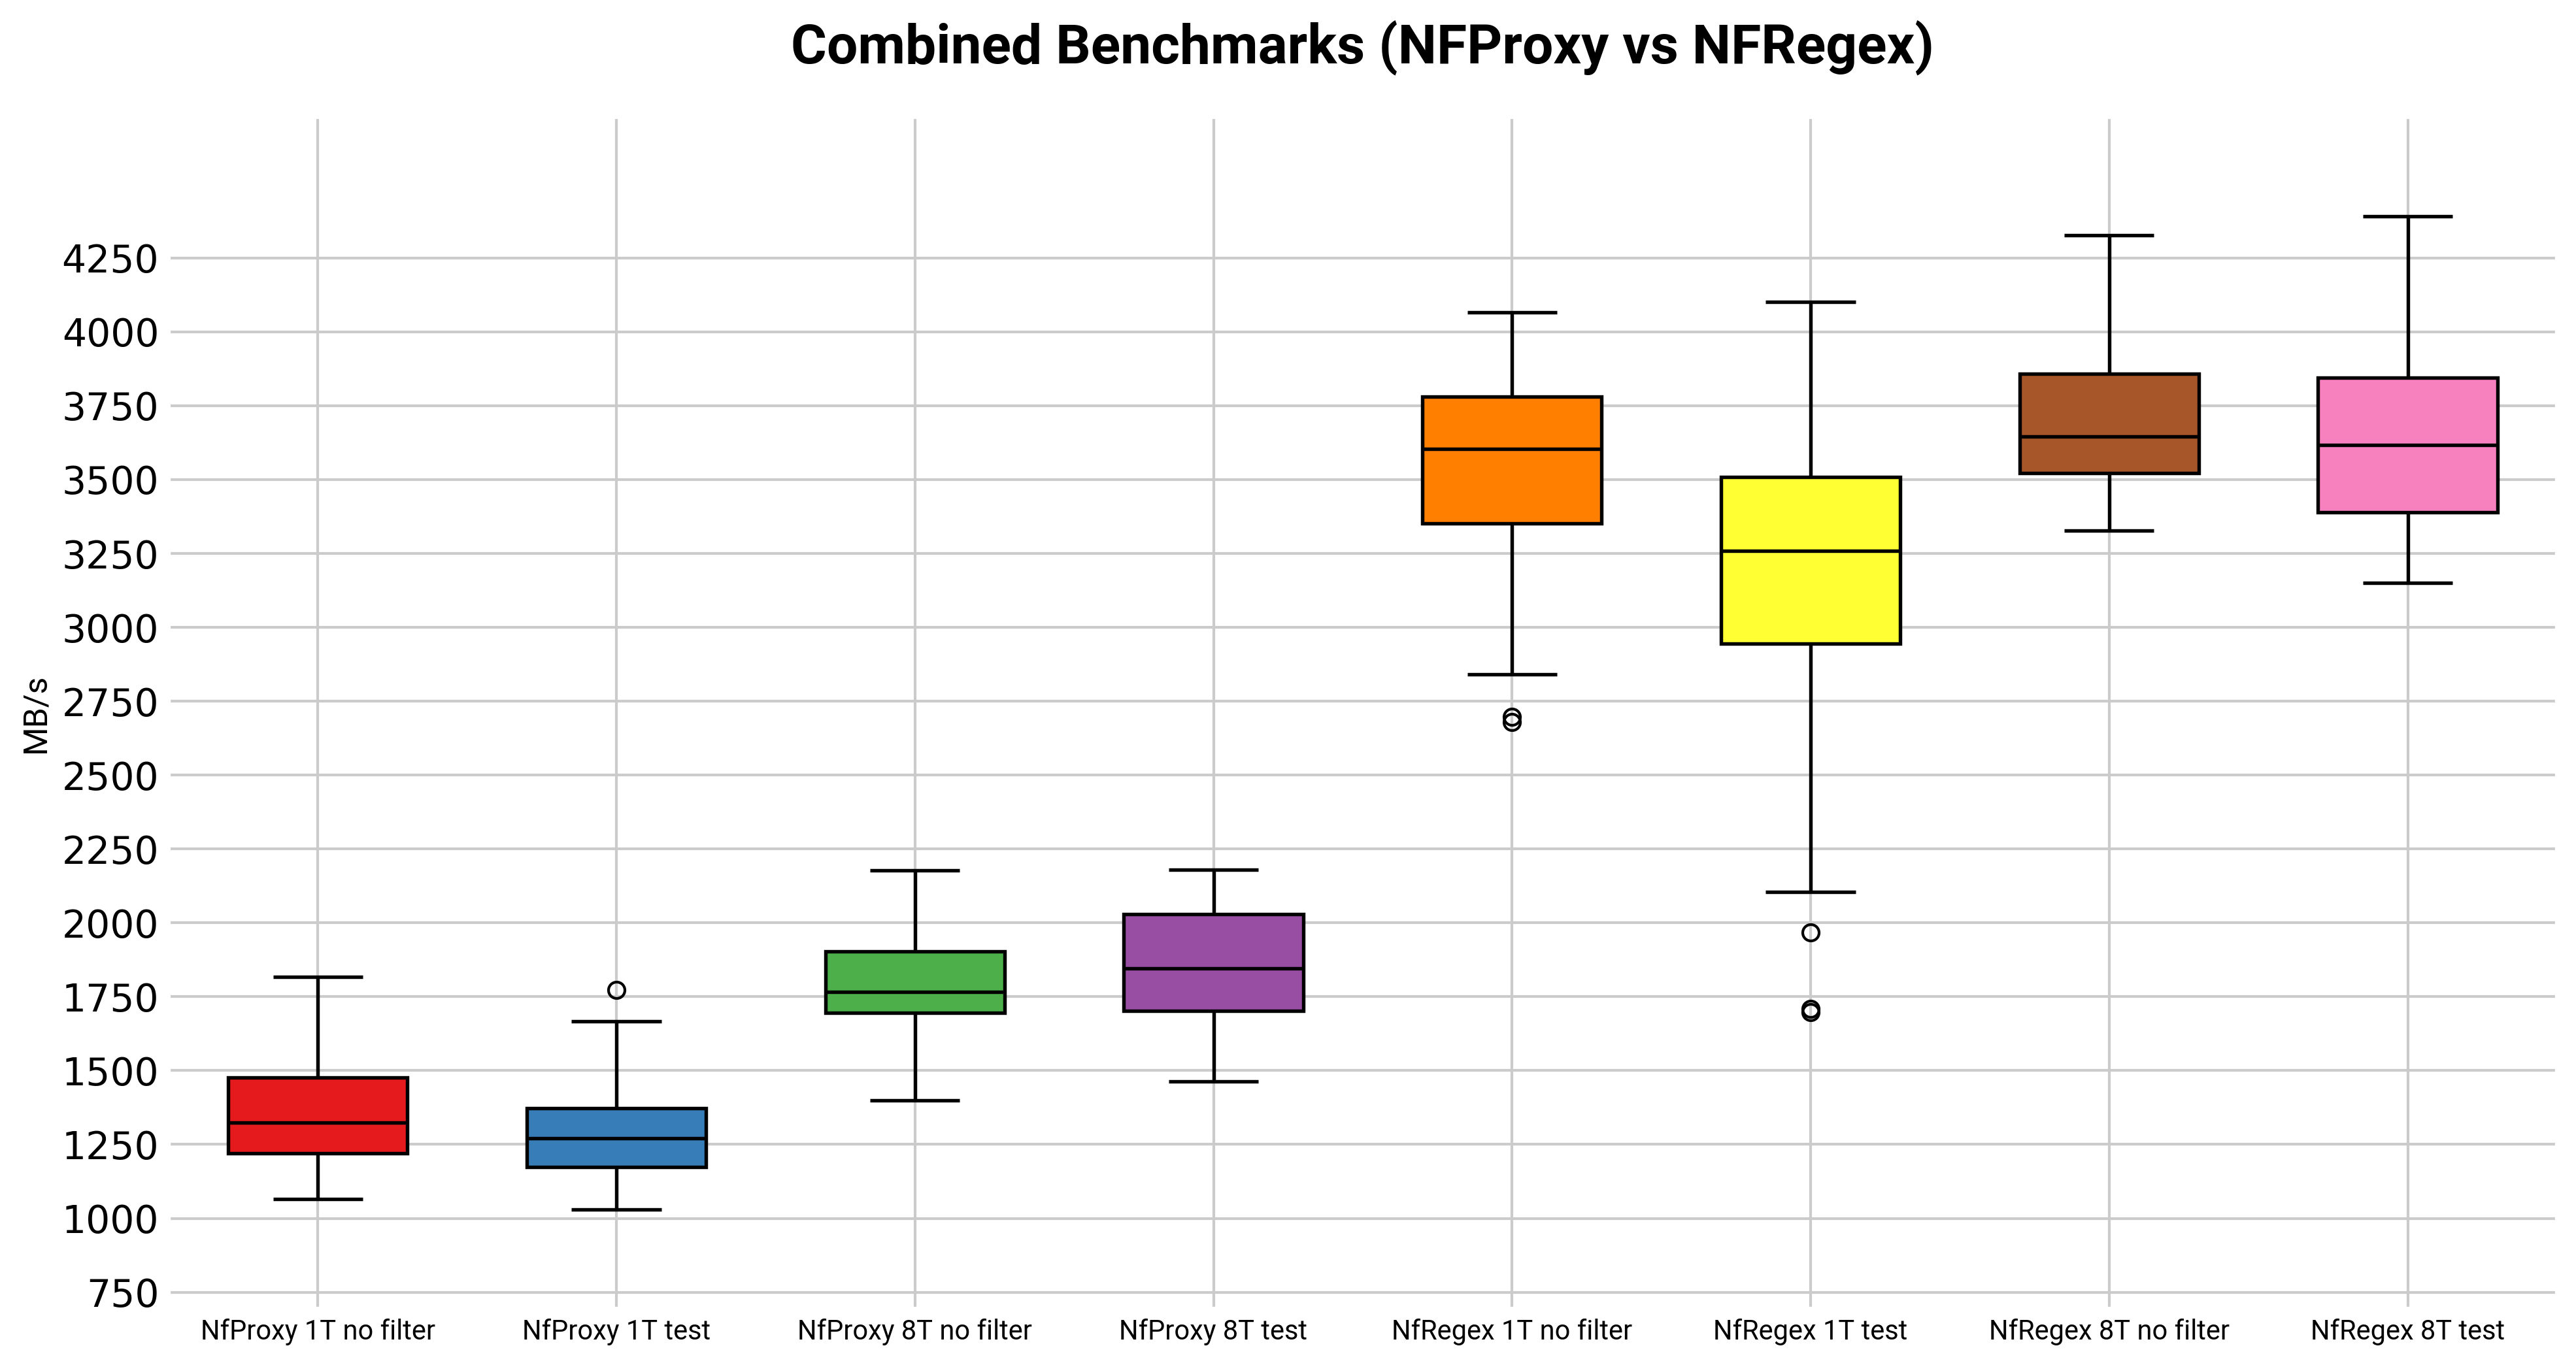
\includegraphics[width=0.98\textwidth]{images/chapter4/whisker_compare.png}
    \caption{Grafico Whisker sulle misure di throughput di nfproxy e nfregex}\label{fig:wisker_nfproxy_nfregex}
\end{figure}

\begin{figure}[H]
    \centering
    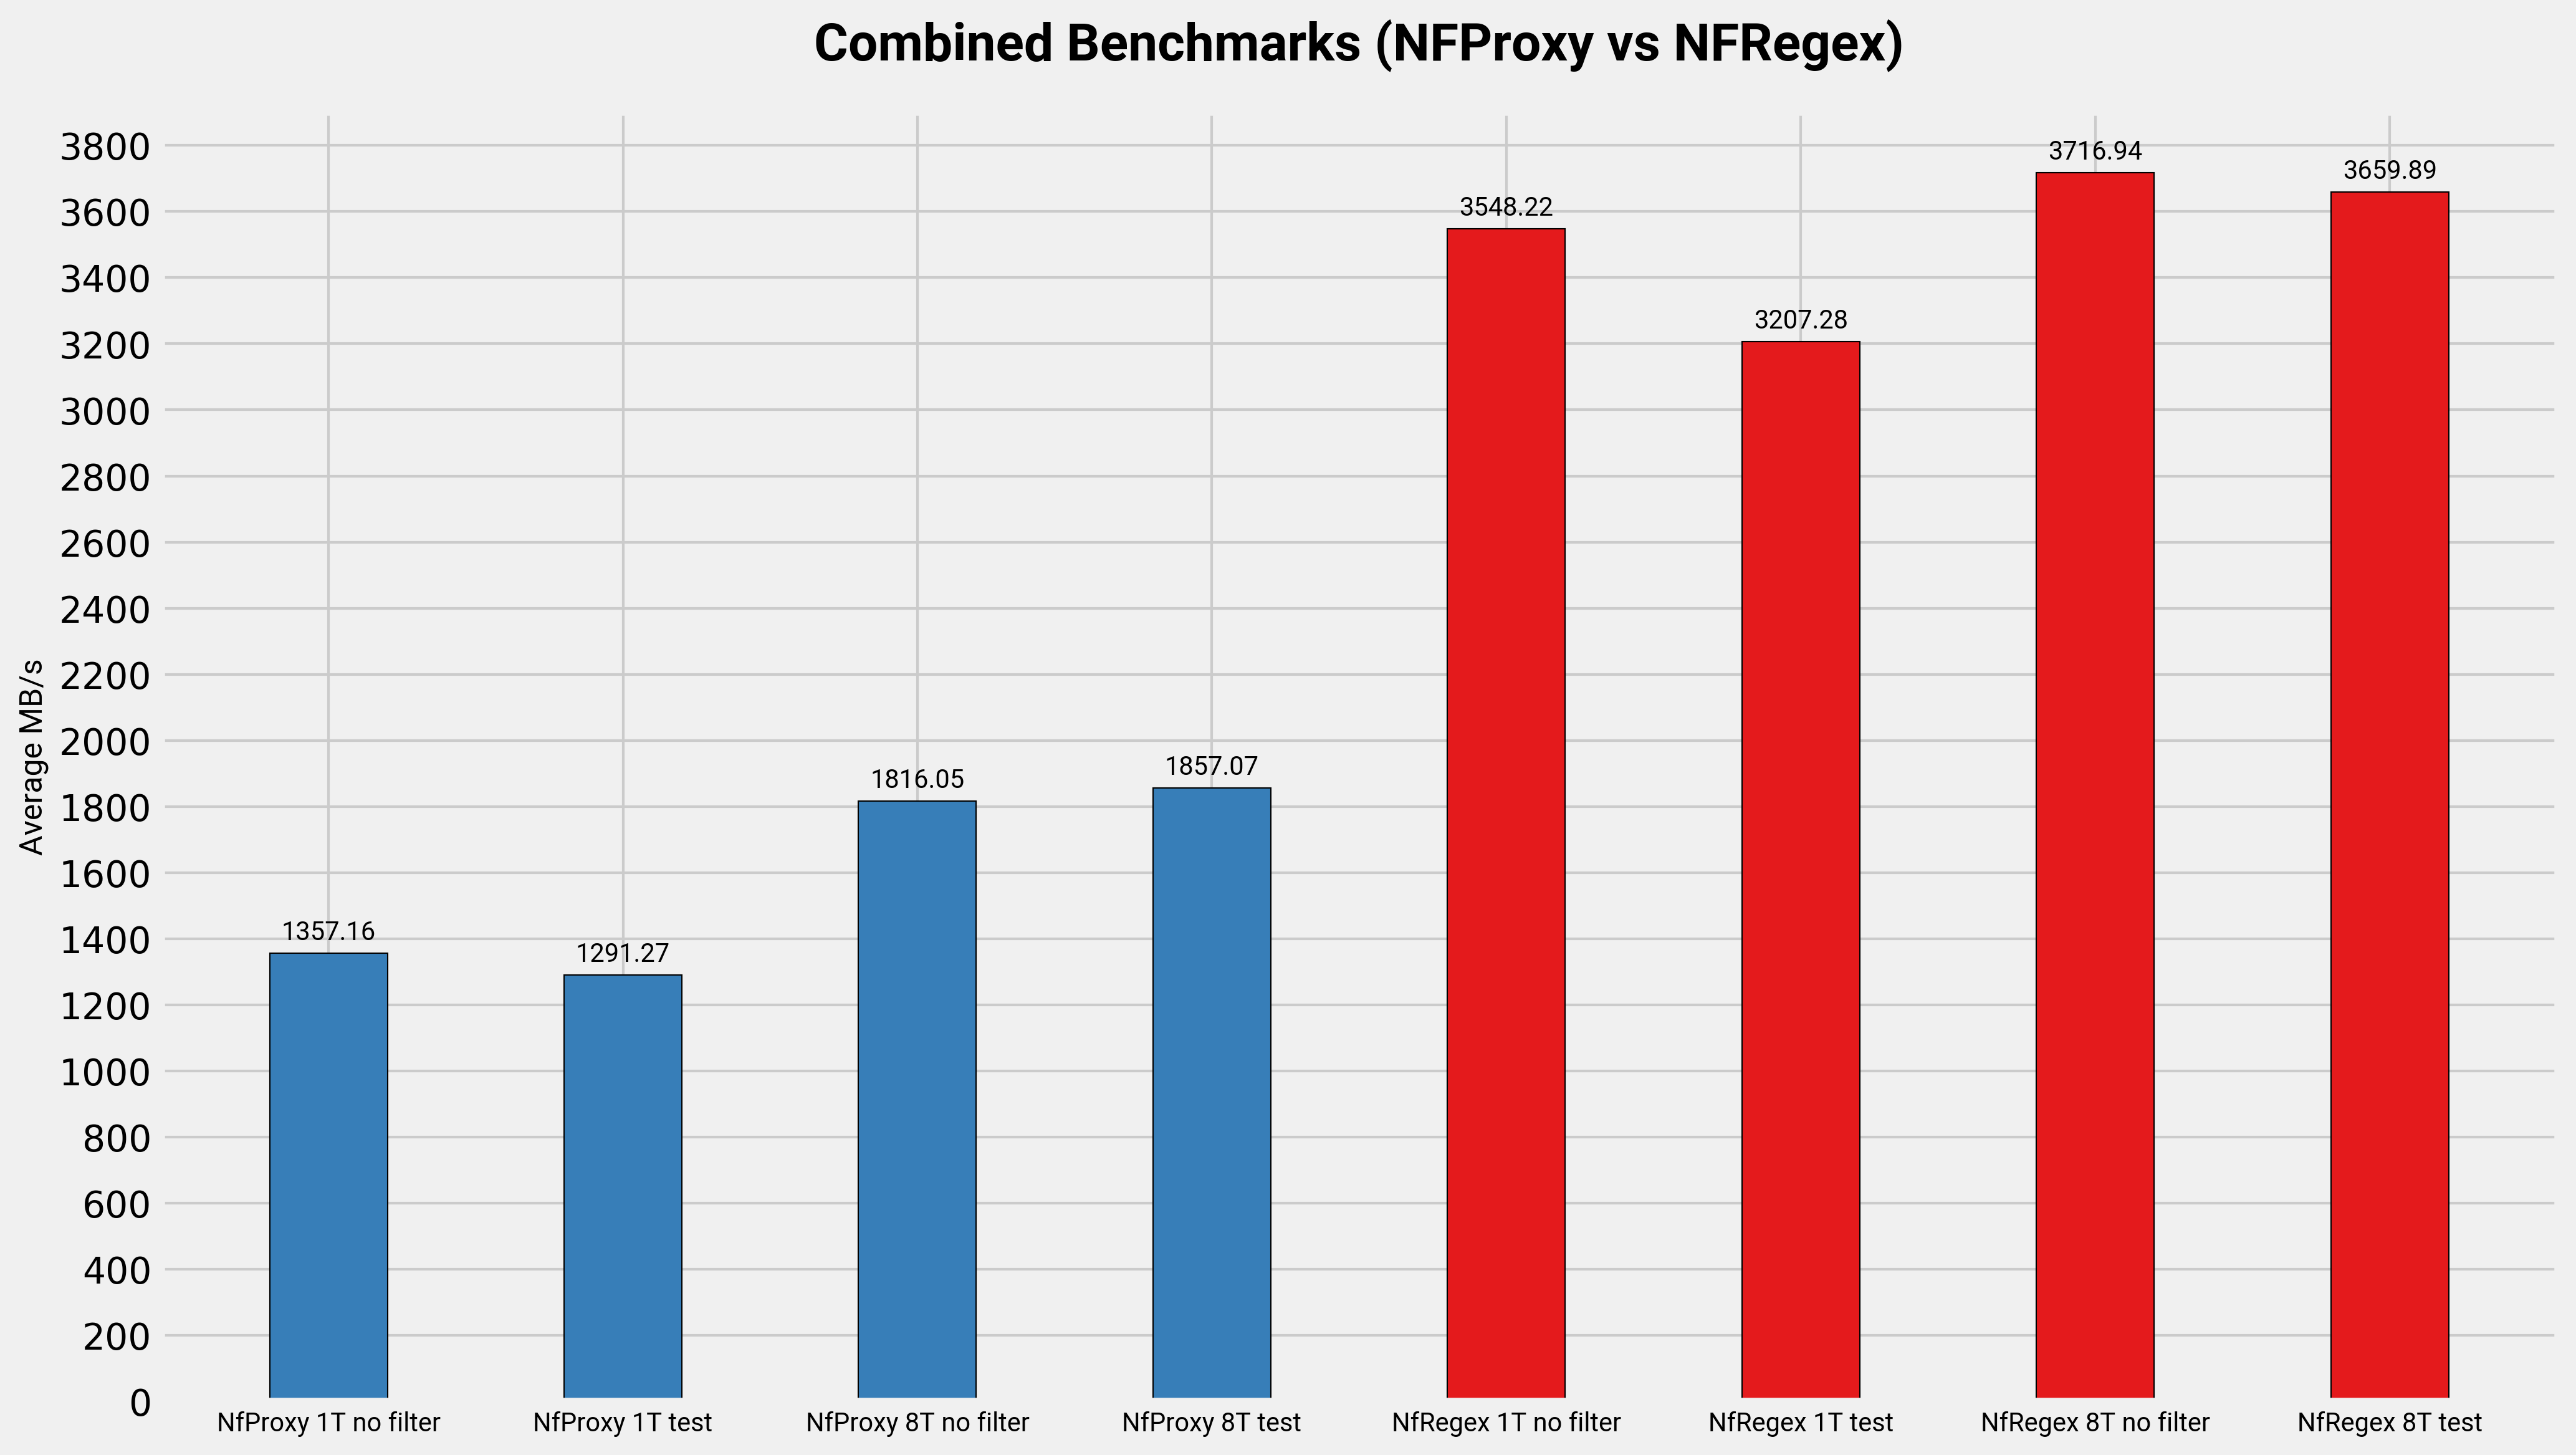
\includegraphics[width=0.98\textwidth]{images/chapter4/istrogramma_compare.png}
    \caption{Istogramma sulle misure medie di throughput di nfproxy e nfregex}\label{fig:istogramma_nfproxy_nfregex}
\end{figure}

Dal confronto di nfproxy e nfregex si può notare come nfproxy abbia un calo di prestazioni rilevante rispetto a nfregex, che tuttavia
rimane comunque abbondantemente alto per supportare anche carichi di rete molto elevati.\\
